\documentclass{article}
\usepackage{amsmath, amssymb}
\usepackage[margin=1in]{geometry}
\usepackage{url}
\usepackage{tikz}

\title{Unit 2 Ext. Problems}
\author{
Greyson Knippel \\[4pt]
MATH 339 --- Gonzaga University \\[4pt]
compiled with \LaTeX{}
}
\date{\today}

\begin{document}
\maketitle

% ===================================================================
\section*{Problem 1: Fourier Analysis}

\subsection*{write-up}

functions can be treated like vectors. the inner product is $\langle f,g\rangle = \int_{-\pi}^{\pi} f(x)g(x)\,dx$
(like a dot product but with an integral). if it's 0, the functions are ``orthogonal.''
a fourier series writes a periodic function in the basis $\{1, \cos x, \sin x, \cos 2x, \dots\}$, and the
coefficients are its coordinates. we didn't cover this in class, so i loosely learned it from:

\begin{itemize}
  \item ``But what is a Fourier series? From heat flow to drawing with circles'' (youtube, 3Blue1Brown) \\
        \url{https://www.youtube.com/watch?v=r6sGWTCMz2k}
  \item more ai tools since i was pretty confused on this one.
\end{itemize}

\subsection*{work}

\textbf{A.}

\textbf{i.}
\[
\langle 1, \cos x\rangle = \int_{-\pi}^{\pi} 1 \cdot \cos x\,dx = \sin x\Big|_{-\pi}^{\pi} = \sin(\pi) - \sin(-\pi) = 0 - 0 = \boxed{0}
\]

\textbf{ii.}
\[
\langle 1, \sin x\rangle = \int_{-\pi}^{\pi} 1 \cdot \sin x\,dx = -\cos x\Big|_{-\pi}^{\pi} = -\cos(\pi) + \cos(-\pi) = -(-1) + (-1) = \boxed{0}
\]

\textbf{iii.} use the identity $\sin x \cos x = \tfrac12 \sin 2x$:
\[
\langle \sin x, \cos x\rangle = \int_{-\pi}^{\pi} \sin x\cos x\,dx = \int_{-\pi}^{\pi} \tfrac12 \sin 2x\,dx
= -\tfrac14\cos 2x\Big|_{-\pi}^{\pi}
\]
\[
= -\tfrac14\cos(2\pi) + \tfrac14\cos(-2\pi) = -\tfrac14(1) + \tfrac14(1) = \boxed{0}
\]
all 0, so they're orthogonal.

\textbf{B.}
\begin{itemize}
  \item[i.] functions with sharp corners/jumps (like a square wave) need infinitely many frequencies, so no finite basis can span the space
  \item[ii.] compression (a few coefficients instead of a whole table), and the coefficients show which cycles drive the data + you can plug in any $t$
  \item[iii.] you can't compute infinitely many terms, so you have to cut it off and its only an approximation
\end{itemize}

\textbf{C.}
\begin{itemize}
  \item[i.] $1,\ \cos(2\pi t/12),\ \cos(2\pi t/24)$. the constant level, a 12 hour tide cycle (twice a day), and a 24 hour cycle (once a day).
  \item[ii.] write $h(t)$ as a linear combination of the basis:
  \[
  h(t) = 2.4\,(1) + 1.8\cos\!\left(\tfrac{2\pi t}{12}\right) + 0.5\cos\!\left(\tfrac{2\pi t}{24}\right)
  \quad\Rightarrow\quad
  \boxed{[h]_B = (2.4,\ 1.8,\ 0.5)}
  \]
  \item[iii.] the average water height (the cosines average to 0)
  \item[iv.] cosine goes between $-1$ and $1$, so each term can move the water by up to its coefficient:
  \[
  \text{12 hr: } 1.8(\pm1) = \pm 1.8 \qquad \text{24 hr: } 0.5(\pm1) = \pm 0.5
  \]
  the 12 hour one, since $1.8 > 0.5$.
\end{itemize}

\textbf{D.}
\begin{itemize}
  \item[i.] $440$, it has the biggest coefficient ($3.5$)
  \item[ii.] drop $0.05$:
  \[
  \boxed{s(t) \approx 3.5\sin(440t) + 1.2\sin(880t) + 0.3\sin(1320t)}
  \]
  the energy (loudness) of each frequency is its coefficient squared. since the basis is orthogonal (part A), the total is the sum:
  \[
  3.5^2 + 1.2^2 + 0.3^2 + 0.05^2 = 12.25 + 1.44 + 0.09 + 0.0025 = 13.7825
  \]
  \[
  \frac{0.0025}{13.7825} \approx 0.00018 \approx 0.02\%
  \]
  so the dropped term is only about $0.02\%$ of the sound, and you cant really hear the difference
\end{itemize}

% ===================================================================
\section*{Problem 2: Principal Component Analysis}

\subsection*{write-up}

PCA is a change of basis where the first new axis points where the data spreads out the most.
if the data barely moves along the other axes, you can drop them and lose almost nothing.
coordinates in $B = \{\mathbf{b}_1, \mathbf{b}_2\}$ come from solving $\mathbf{x} = c_1\mathbf{b}_1 + c_2\mathbf{b}_2$.
we didn't cover this in class, so i loosely learned it from:

\begin{itemize}
  \item ``StatQuest: Principal Component Analysis (PCA), Step-by-Step'' (youtube) \\
        \url{https://www.youtube.com/watch?v=FgakZw6K1QQ}

    \item ai tools to explain the rest since i was pretty confused.
\end{itemize}

\subsection*{work}

\textbf{A.}

\textbf{i.} (math, reading):
$A = (520,510),\ B = (580,590),\ C = (610,620),\ D = (680,690),\ E = (740,730)$

\textbf{ii. \& iv.}

\begin{center}
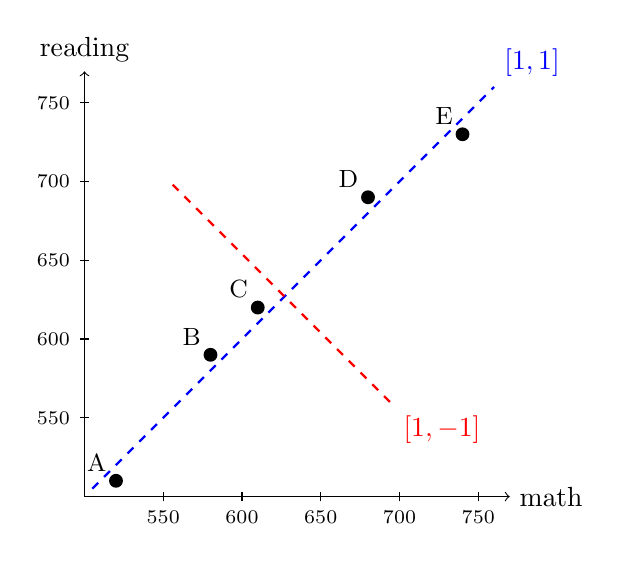
\begin{tikzpicture}[x=0.02cm, y=0.02cm]
  \begin{scope}[shift={(-500,-500)}]
    \draw[->] (500,500) -- (770,500) node[right] {math};
    \draw[->] (500,500) -- (500,770) node[above] {reading};
    \foreach \t in {550,600,650,700,750} {
      \draw (\t,497) -- (\t,503); \node[below] at (\t,497) {\scriptsize\t};
      \draw (497,\t) -- (503,\t); \node[left] at (497,\t) {\scriptsize\t};
    }
    \draw[dashed, blue, thick] (505,505) -- (760,760) node[above right] {$[1,1]$};
    \draw[dashed, red, thick] (556,698) -- (696,558) node[below right] {$[1,-1]$};
    \foreach \p/\q/\l in {520/510/A, 580/590/B, 610/620/C, 680/690/D, 740/730/E} {
      \fill (\p,\q) circle (2.5pt);
      \node[above left] at (\p,\q) {\small \l};
    }
  \end{scope}
\end{tikzpicture}
\end{center}

\textbf{ii.} points almost lie on $y = x$. high math $\to$ high reading

\textbf{iii.} no, they spread along $y=x$ but barely perpendicular to it

\textbf{iv.} $[1,1]$

\textbf{v.}
\[
c_1 + c_2 = m,\quad c_1 - c_2 = r
\quad\Rightarrow\quad
c_1 = \tfrac{m + r}{2},\quad c_2 = \tfrac{m - r}{2}
\]
\[
\begin{aligned}
A&:\ c_1 = \tfrac{520 + 510}{2} = \tfrac{1030}{2} = 515, & c_2 &= \tfrac{520 - 510}{2} = \tfrac{10}{2} = 5 \\
B&:\ c_1 = \tfrac{580 + 590}{2} = \tfrac{1170}{2} = 585, & c_2 &= \tfrac{580 - 590}{2} = \tfrac{-10}{2} = -5 \\
C&:\ c_1 = \tfrac{610 + 620}{2} = \tfrac{1230}{2} = 615, & c_2 &= \tfrac{610 - 620}{2} = \tfrac{-10}{2} = -5 \\
D&:\ c_1 = \tfrac{680 + 690}{2} = \tfrac{1370}{2} = 685, & c_2 &= \tfrac{680 - 690}{2} = \tfrac{-10}{2} = -5 \\
E&:\ c_1 = \tfrac{740 + 730}{2} = \tfrac{1470}{2} = 735, & c_2 &= \tfrac{740 - 730}{2} = \tfrac{10}{2} = 5
\end{aligned}
\]
\[
\boxed{A = (515, 5),\ B = (585, -5),\ C = (615, -5),\ D = (685, -5),\ E = (735, 5)}
\]
check A: $515(1,1) + 5(1,-1) = (515 + 5,\ 515 - 5) = (520,510)$. \checkmark

spread along each axis:
\[
[1,1]:\ 735 - 515 = 220 \qquad [1,-1]:\ 5 - (-5) = 10
\]
the $[1,-1]$ coordinates are all $\pm 5$, basically nothing compared to the $[1,1]$ ones

\textbf{vi.} $[1,1]$ = overall performance ($c_1$ is the average). $[1,-1]$ = math vs reading difference
yes more useful, one number ranks students and the other shows if they are lopsided

\textbf{vii.} $[1,1]$, you only lose $\pm5$ points

\textbf{B.}
\begin{itemize}
  \item[i.] 20 before, 2 after.
  \item[ii.] less storage, faster, and you can actually plot 2 coordinates. for example with 1000 samples:
  \[
  \text{before: } 1000 \times 20 = 20{,}000 \text{ numbers}
  \qquad
  \text{after: } 1000 \times 2 = 2{,}000 \text{ numbers}
  \]
  (plus the 2 basis vectors, $2 \times 20 = 40$ numbers), so about 10 times less.
\end{itemize}

\textbf{C.} using $[1,1]$ (total) and $[1,-1]$ (preference): $c_1 = \frac{\text{TV}+\text{movies}}{2}$, $c_2 = \frac{\text{TV}-\text{movies}}{2}$
\[
\begin{aligned}
A&:\ c_1 = \tfrac{2 + 3}{2} = 2.5, & c_2 &= \tfrac{2 - 3}{2} = -0.5 \\
B&:\ c_1 = \tfrac{4 + 4}{2} = 4, & c_2 &= \tfrac{4 - 4}{2} = 0 \\
C&:\ c_1 = \tfrac{6 + 7}{2} = 6.5, & c_2 &= \tfrac{6 - 7}{2} = -0.5 \\
D&:\ c_1 = \tfrac{8 + 9}{2} = 8.5, & c_2 &= \tfrac{8 - 9}{2} = -0.5 \\
E&:\ c_1 = \tfrac{10 + 11}{2} = 10.5, & c_2 &= \tfrac{10 - 11}{2} = -0.5
\end{aligned}
\]
\begin{itemize}
  \item[i.] total viewing. spread: $10.5 - 2.5 = 8$ vs $0 - (-0.5) = 0.5$
  \item[ii.] total viewing
  \item[iii.] TV vs movies. user B stands out ($c_2 = 0$, everyone else $-0.5$)
  \item[iv.] yes, it splits ``how much'' from ``what they watch'' and nothing is lost (just a change of basis)
\end{itemize}

% ===================================================================
\section*{Problem 4: Cryptography}

\subsection*{write-up}

mod 5 means keep the remainder after dividing by 5. since 5 is prime, every number that isnt zero has an inverse,
so $\mathbb{Z}_5^2$ works like a normal vector space (just reduce mod 5)
encrypting = multiply the message by a secret invertible matrix, decrypting = multiply by the inverse.
we didn't cover this in class, so i loosely learned it from:

\begin{itemize}
  \item this one i was already familiar with modular, but i used ai tools to explain the rest.
\end{itemize}

\subsection*{work}

\textbf{A.}
divide by 5 and keep the remainder:

\textbf{i.} $3 + 4 = 7 = 1(5) + 2 \equiv \boxed{2} \pmod 5$

\textbf{ii.} $4 + 4 = 8 = 1(5) + 3 \equiv \boxed{3} \pmod 5$

\textbf{iii.} $3 \cdot 4 = 12 = 2(5) + 2 \equiv \boxed{2} \pmod 5$

\textbf{iv.} try every value:
\[
2(0) = 0,\quad 2(1) = 2,\quad 2(2) = 4,\quad 2(3) = 6 = 1(5) + 1 \equiv 1,\quad 2(4) = 8 \equiv 3
\]
\[
\boxed{x = 3}
\]

\textbf{B.}
\textbf{i.} 5 choices for the first entry and 5 for the second: $5 \times 5 = \boxed{25}$ vectors

\textbf{ii.} $(2,4) + (3,2) = (2 + 3,\ 4 + 2) = (5, 6) \equiv \boxed{(0,1)}$

\textbf{iii.} $3(1,4) = (3 \cdot 1,\ 3 \cdot 4) = (3, 12) \equiv \boxed{(3,2)}$

\textbf{C.}

\textbf{i.} $c_1(1,0) + c_2(0,1) = (c_1, c_2) = (0,0) \Rightarrow c_1 = c_2 = 0$, so independent
2 independent vectors in a 2-dim space, so yes its a basis

\textbf{ii.} $(3,4) = 3\mathbf{v}_1 + 4\mathbf{v}_2 \Rightarrow \boxed{(3,4)}$

\textbf{iii.}
\[
\left[\begin{array}{cc|c} 1 & 1 & 3 \\ 1 & 2 & 4 \end{array}\right]
\xrightarrow{R_2 - R_1}
\left[\begin{array}{cc|c} 1 & 1 & 3 \\ 0 & 1 & 1 \end{array}\right]
\xrightarrow{R_1 - R_2}
\left[\begin{array}{cc|c} 1 & 0 & 2 \\ 0 & 1 & 1 \end{array}\right]
\Rightarrow \boxed{(2,1)}
\]
check: $2(1,1) + 1(1,2) = (2 + 1,\ 2 + 2) = (3,4)$. \checkmark

(also $\det\begin{bmatrix}1&1\\1&2\end{bmatrix} = 1(2) - 1(1) = 1 \not\equiv 0$, so $\mathbf{u}_1, \mathbf{u}_2$ is a basis)

same vector, different coordinates

\textbf{iv.} if you only see $(2,1)$ and dont know the basis, you dont know it means $(3,4)$ the basis is the key

\textbf{D.}
\[
\begin{bmatrix}1&2\\3&1\end{bmatrix}\begin{bmatrix}1\\2\end{bmatrix}
=
\begin{bmatrix}1(1) + 2(2) \\ 3(1) + 1(2)\end{bmatrix}
=
\begin{bmatrix}5\\5\end{bmatrix}
\equiv \boxed{\begin{bmatrix}0\\0\end{bmatrix}}
\]
\[
\begin{bmatrix}1&2\\3&1\end{bmatrix}\begin{bmatrix}3\\4\end{bmatrix}
=
\begin{bmatrix}1(3) + 2(4) \\ 3(3) + 1(4)\end{bmatrix}
=
\begin{bmatrix}11\\13\end{bmatrix}
=
\begin{bmatrix}2(5) + 1 \\ 2(5) + 3\end{bmatrix}
\equiv \boxed{\begin{bmatrix}1\\3\end{bmatrix}}
\]
$A$ has to be invertible mod 5 ($\det A \not\equiv 0$). but
\[
\det A = 1(1) - 2(3) = 1 - 6 = -5 \equiv 0 \pmod 5
\]
so this $A$ does NOT work: $(1,2)$ and $(0,0)$ both encode to $(0,0)$, so you cant get $(1,2)$ back

\textbf{E.}
\begin{itemize}
  \item[i.] 100 (each one is a byte, 0--255)
  \item[ii.] 257 is prime, so every nonzero number has an inverse. in $\mathbb{Z}_{256}$ even numbers dont, so matrix inverses can fail. example with 2:
  \[
  \mathbb{Z}_{257}:\ 2(129) = 258 = 1(257) + 1 \equiv 1, \text{ so } 2^{-1} = 129
  \]
  \[
  \mathbb{Z}_{256}:\ 2x \text{ is always even, and } 2(128) = 256 \equiv 0, \text{ so } 2x \not\equiv 1 \text{ for any } x
  \]
  \item[iii.] messages are vectors, the standard basis is the plain message, and the secret basis is the key. encrypt = change to the secret basis, decrypt = change back.
  \item[iv.] matrices are how you do a change of basis, they mix all the characters together (harder to crack), and decrypting is multiplying by $A^{-1}$???
\end{itemize}

\end{document}
